%!TEX root = ../thesis.tex
\section{要求仕様}
前項で設定した作業と既存のオフィスロボットの調査を基に,要求仕様を決定する.以下に決定した要求仕様とその理由を示す.
\begin{itemize}
  \item アームリーチ70cm程度
  \item 軽量化
  \item 6自由度
  \begin{itemize}
    \item 肩2軸(ヨー,ピッチ)
    \item 肘1軸(ロール)
    \item 手首3軸(ヨー,ピッチ,ロール)
  \end{itemize}
  \item 可搬重量500g以上
  \item 平行グリッパ
  \item QDDモータを使用
\end{itemize}
\subsection{アームのサイズ}
ロボットアームのサイズは,オフィス環境で活動するのに適したサイズが好ましい.既存のオフィスロボットのアームリーチは,平均約70cm程度である.また,前項で設定した作業より,対象物の設置位置と箱の設置位置は50cm以内の位置であるため,アームリーチ70cm程度あれば作業の遂行も可能である.
\subsection{アーム重量}
既存のオフィスロボットのアームの重量は調査してもわからなかったが,将来的に台車ロボットに搭載することや,双腕ロボットにすることを考えると,軽量であることが望ましい.また,軽量化することで安全性にも寄与すると考えられる.
\subsection{アームの自由度}
自由度の決定は既存のオフィスロボットを参考に行う.既存のオフィスロボットの自由度を調査した結果を示す.7自由度と6自由度のロボットがほとんどである.6自由度に比べ7自由度は柔軟な操作が可能であるが,アーム重量が増加し,コストも高くなる.そのため,6自由度のアームが望ましい.この際,軸配置についても既存のロボットアームを参考に,肩2軸(ヨー,ピッチ),肘1軸(ロール),手首3軸(ヨー,ピッチ,ロール)とする.

\begin{figure}[h]
  \centering
  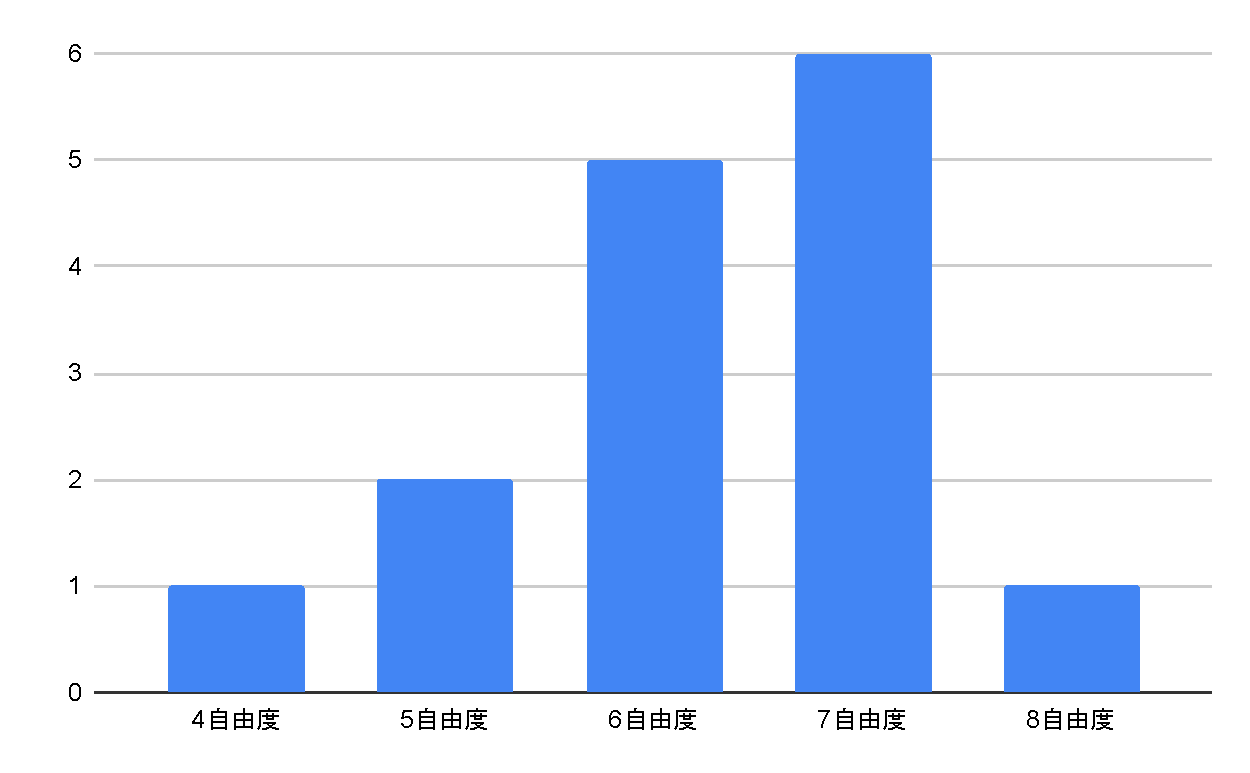
\includegraphics[width=10cm]{images/armDof.pdf}
  \caption{既存のオフィスロボットの自由度}
  \label{fig:armDof}
\end{figure}

\subsection{可搬重量}
設定した作業では,500g以下の対象物を把持する.そのため,アームの可搬重量は500g以上であることが望ましい.
\subsection{エンドエフェクタ}
既存のオフィスロボットのエンドエフェクタは,Mobile ALOHAに搭載されているロボットアーム(\ref{fig:alohaarm}に示す)のような平行グリッパが多く,様々な形状の物体を把持していることが確認できた.そのため,本研究で開発するアームにも平行グリッパを搭載する.

\begin{figure}[h]
  \centering
  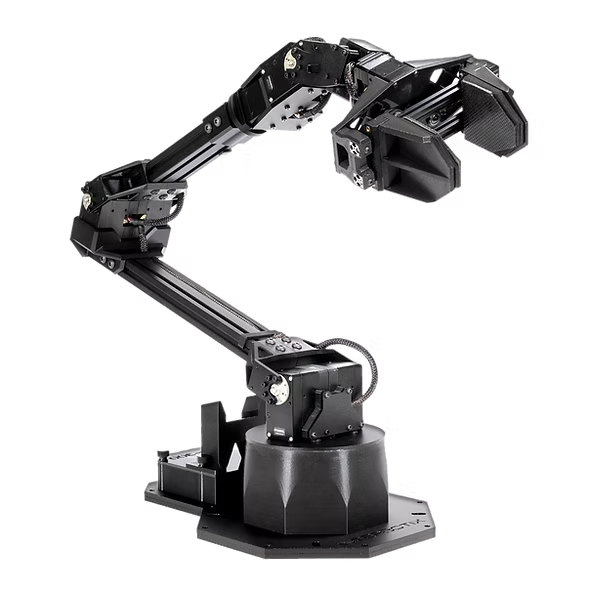
\includegraphics[width=10cm]{images/alohaarm.png}
  \caption{Mobile ALOHO Arm}
  \label{fig:alohaarm}
\end{figure}

\subsection{安全性}
オフィス環境には多くの人がいるため、ロボットアームが人に接触する可能性があり、安全性が重要である。既存のオフィスロボットで使用されているアクチュエータは、高減速比でバックドライバビリティが低いものが多い。そのため、低減速比のQDDモータを使用することで、バックドライバビリティを高め、衝突時に柔軟な関節を実現することができる。そもそも,利用者や近くの人間に危害を加えないことが重要であり,QDDモータを使用する以外にも対策を講じる必要がある.
\newpage